\documentclass[english,master]{swsLeipzig}
% When you change the language, pdflatex may halt on recompilation.
% Just hit enter to continue and recompile again. This should fix it.

%
% Values
% ------
\ThesisSetTitle{RAGBench - A Benchmark Framework for Retrieval-Augmented Generation Systems}
\ThesisSetKeywords{RAG, benchmarking} % only for PDF meta attributes

\ThesisSetAuthor{Jan Albrecht}
\ThesisSetStudentNumber{3772326}
\ThesisSetDateOfBirth{17}{2}{1995}
\ThesisSetPlaceOfBirth{Freital}

\ThesisSetSupervisors{Prof.\ Dr.\ Norbert Siegmund,Prof.\ Dr.\ Unknown Yet}

\ThesisSetSubmissionDate{31}{1}{2025}

%
% Suggested Packages
% ------------------
\usepackage[sort&compress]{natbib}
%   Allows citing in different ways (e.g., only the authors if you use the
%   citation again within a short time).

% Let us get started by citing \citet{manning:1999}!
% So what did \citeauthor{manning:1999} do in \citeyear{manning:1999}?
% Good question!



%
\usepackage{booktabs}
%    For tables ``looking the right way''.
%
%\usepackage{tabularx}
%    Enables tables with columns that automatically fill the page width.
%
%\usepackage[ruled,algochapter]{algorithm2e}
%    A package for pseudo code algorithms.
%
%\usepackage{amsmath}
%    For tabular-style formatting of mathematical environments.
%

%
% Commenting (by your supervisor)
% -------------------------------
\usepackage{xcolor}
\usepackage{soul}

% Graphical packages
\usepackage{graphicx}
\newcommand{\bscom}[2]{%
  % #1 Original text.
  % #2 Replacement text.
    \st{\scriptsize\,#1}{\color{blue}\scriptsize\,#2}%
  }
  
  \newcommand{\boldred}[1]{\textbf{\textcolor{red}{#1}}}
% Create links in the pdf document
% Hyperref has some incompatibilities with other packages
% Some other packages must be loaded before, some after hyperref
% Additional options to the hyperref package can be provided in the braces []
\usehyperref[backref] % This will add back references in the bibliography

\begin{document}
\begin{frontmatter}
  \begin{abstract}
    A short summary.
  \end{abstract}

  \tableofcontents

  %\chapter*{Acknowledgements} % optional
  %I thank the authors of the swsLeipzig template for their excellent work!

  %\listoffigures % optional

  %\listoftables % optional

  %\listofalgorithms % optional
  %    requires package algorithm2e

  % optional: list of symbols/notation (e.g., using the nomencl package)
\end{frontmatter}

\chapter{Introduction}\label{introduction}
The year 2017 can be stated as the beginning of the interesting journey of artificial intelligent language models. With the publication of "Attention is all you need" from Vaswani \cite{vaswani2023attentionneed} the rapid development of language models and later large language models (LLMs) took off.

Today there is a variety of real world products that are using this technology, such as content generators like ChatGPT \cite{OpenAI_2022} or Claude \cite{Anthropic_2023}, translators like DeepL \cite{DeepL_SE} and Coding Assistants like Github Copilot \cite{Friedman_2022}. The list can be expanded with technologies like sentiment analysis, question answering systems, market research or education systems. Open-source models are available for each of these technologies, providing strong alternatives to proprietary services.

The remarkable capacity of large language models has led to wide acceptance in society. However LLMs have fundamental problems that cannot be solved with more training or larger models. Training models frequently is expensive, so daily training isn't feasible. Therefore every new information such as elections, weather or sport results that occurred between the last training and the user prompt are unknown to the model. On top of that, models can only be trained on available data. Private information of users that might be relevant for the prompt are not considered in the generation process. LLMs struggle also with long-tail information, which occurs rarely in the training data \cite{Kandpal.15.11.2022}.

When information is missing or underrepresented, outputs will deviate from user inputs, repeat previous outputs or may be made up by the LLM \cite{Zhang.03.09.2023}. This technology is already used in many sectors with billions of customers such as marketing, retail and eCommerce, education, healthcare, finance and law and media. It is crucial to develop systems that are as correct as possible.

The solution to potential missing information in training is to provide all necessary information to the LLM beforehand within the prompt, so that the generator just has to construct a coherent text for the user. This can be achieved with so-called Retrieval-Augmented Generation Systems (RAGs), where the raw user prompt is used to retrieve relevant data from a database that gets summarised and inserted into the prompt for the generator. This method overcomes many of the challenges LLMs face. Data can be accessed from private and up-to-date sources. The frequency of information occurrences no longer matters as long as the database includes it for retrieval. For having recent information, it is no longer required to train the underlying model.
% cite original RAG Paper
% cite paper that shows the advantages of RAG

However, the adoption of RAG systems introduces significant overhead and complexity. The system requires additional steps between the prompt request and output. Most of those steps can not be parallelized. That results in longer inference times and also leads to the more resource intensive system. Next to the increasing infrastructure costs, developing and maintaining a RAG is more time consuming than developing a LLM, because the LLM is a part of the larger system. RAGs are not by default significantly better systems than pure LLMs as Simon \cite{Simon.10112024} showed. These complex systems are highly sensitive to small configuration changes.

Therefore there is an important question to be asked: 
\begin{quotation}
    "Is an advanced RAG system necessary for your use case, or is a standalone LLM sufficient?"
\end{quotation}
\begin{quotation}
    "Is your RAG the best one for your specific use-case?"
\end{quotation}

The answers to these questions are hard to find, because you have to implement a RAG, to test it on your problem and your data. The scientific landscape of Retrieval-Augmented Generation Systems is a vast community with rapid development. Staying up-to-date with that research topic is time consuming for companies and research departments. 

The implementation of the RAG is just one part of the decision process. It is difficult to evaluate LLMs and all systems that are based on that technology, because outputs are not deterministic and such models are like a black-box. It is not obvious why the model responds with a certain output. Another problem is that there is a whole set of potential correct answers, because text-based outputs can have many forms. Lets consider following example:\\

Question: \textit{Is the evaluation process of LLMs an easy task?}\\
Answer 1: \textit{The evaluation process of LLMs is not an easy task.}\\
Answer 2: \textit{No, the evaluation process is a difficult task.}\\[6pt]

Both answers are correct, but which metric must be used to measure this outcome? 

The Evaluation of RAGs is even harder, because it has the same problems next to its own ones. RAGs are complex and is composed of many parts. Each part can lead to errors and therefore all components of the systems need to be evaluated next to an end-to-end evaluation of the whole system as Salemi \cite{Salemi.2024} and Yu \cite{Yu.2024} showed.

There are companies and research groups that successfully solved parts of this problem with developing tools, frameworks and libraries such as AutoRAG \cite{AutoRAG}, Llama-Index \cite{Liu_LlamaIndex_2022}, LangChain \cite{Chase_LangChain_2022}, RaLLe \cite{ralle}, FlashRAG \cite{FlashRAG}, RAGLAB \cite{zhang-etal-2024-raglab}, Haystack \cite{Pietsch_Haystack_the_end-to-end_2019} and FastRAG \cite{Izsak_fastRAG_Efficient_Retrieval_2023}. While an in-depth analysis will follow later in this thesis, it can be stated that all of those tools and frameworks are focussed on developing RAG-Variants, make them production-ready or evaluating them for performance, ignoring the fact that RAGs must be measured for hardware metrics like latency, inference time and CPU usage to determine if the benefits in performance compensate the disadvantages. Additional to this, Simon \cite{Simon.10112024} showed there is lack of external validity in the development of RAGs, because the iterative reconfiguration of those systems that leads to the best performance is a hyperparameter tuning process that overfits the model to the tested data and therefore requires a dataset split with a validation dataset and a holdout test dataset, which is only used to estimate the generalization error.

With this master thesis, we will make two contributions to the scientific landscape of RAGs: (i) A novel benchmarking framework, RAGBench, following the systematic blueprint shown by Simon \cite{Simon.10112024} and evaluating hardware metrics alongside SOTA performance evaluations, (ii) A practical demonstration of RAGBench through an experiment on the software engineering task of configuration validation. For (i), the framework will extend Haystack \cite{Pietsch_Haystack_the_end-to-end_2019} next to the FastRAG library \cite{Izsak_fastRAG_Efficient_Retrieval_2023}. Haystack is an open-source framework for LLMs, RAGs and SOTA search systems. FastRAG builds upon Haystack and adds special RAG architectures. 

The primary results of this work indicate that while RAG systems offer a powerful approach to overcoming LLM limitations, their effective implementation is non-trivial. The development of RAGBench highlighted the critical necessity of incorporating rigorous machine learning practices, such as a strict validation-test split, into RAG evaluation to mitigate overfitting. Furthermore, the application of RAGBench to software configuration validation revealed that retrieval quality is often the predominant bottleneck, and complex RAG architectures do not automatically surpass well-prompted standalone LLMs without careful, task-specific optimization of the retrieval components. Our experiments achieved a competitive F1-score of 0.776 for configuration validation using a standalone model with a Ciri-like few-shot setup, underscoring the importance of robust baselines.

This thesis concludes that a systematic and holistic benchmarking approach, as facilitated by RAGBench, is indispensable for advancing RAG technology. It enables data-driven decisions, helping to determine if a RAG system is truly necessary and how to best configure it for a specific use-case, moving beyond ad-hoc tuning towards more principled and reliable RAG solutions.

This thesis is structured as follows:
Chapter \ref{chap:background} provides an overview of the foundational concepts, including Large Language Models, text retrieval techniques, and the architecture of Retrieval-Augmented Generation systems.
Chapter \ref{chap:relwork} discusses existing research and tools related to RAG evaluation and benchmarking.
Chapter \ref{chap:design} details the design and methodology of the RAGBench framework, emphasizing its core principles for achieving generalizable and reproducible RAG experiments.
Chapter \ref{chap:Experiment} presents a practical application of RAGBench, detailing an experiment focused on using RAG for software configuration validation, and analyzes the obtained results.
Finally, Chapter \ref{chap:Conclusion} summarizes the contributions of this thesis and discusses the implications of RAGBench for future research and development in the field of retrieval-augmented generation.


\chapter{Background}\label{background}


\section{Large Language Models}\label{llm}
LLMs are deep neural network models trained on large corpora of text data. They are predominantly based on the Transformer architecture \cite{Wolf.09.10.2019}. Understanding Large Language Models and their hyperparameters like temperature or top-p is crucial for the development of RAG applications. Below, we explain the Transformer architecture and its main components.

\subsection{Transformer Architecture}
There are many well-known models based on the Transformer architecture, such as BERT, GPT-3.5, LLaMA, and others \cite{Yin.2024}. The Transformer architecture was introduced by Vaswani et al. in 2017. It's based on the self-attention mechanism, which allows the model to weigh the importance of each word in a sentence. The architecture has been shown to outperform other architectures in various NLP tasks.

% include graphic of Transformer architecture
\begin{figure}[!ht]
    \centering
    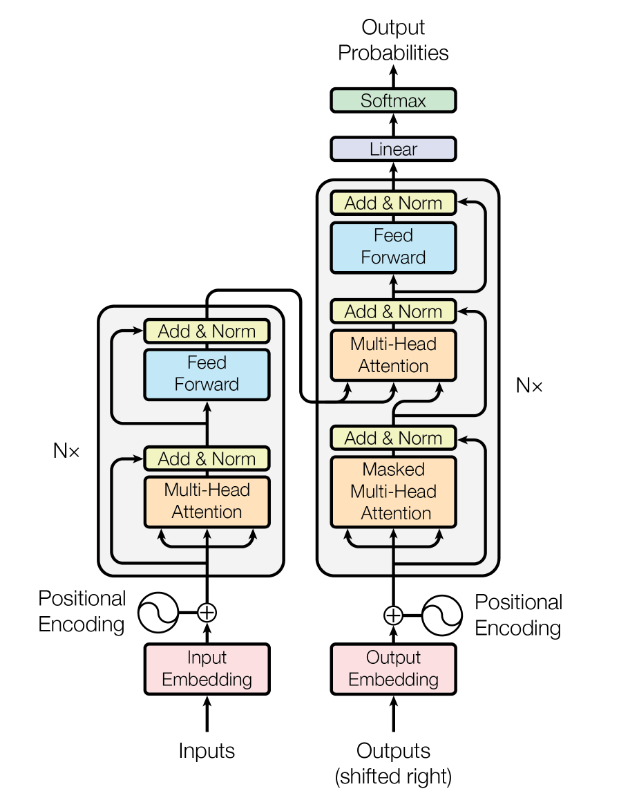
\includegraphics[width=0.6\textwidth]{images/transformers_architecture.png}
    \caption{Transformer Architecture with encoder (left) and decoder (right), Source: Vaswani \cite{vaswani2023attentionneed}}
    \label{fig:transformer_architecture}
\end{figure}

Figure \ref{fig:transformer_architecture} illustrates the Transformer architecture. Both encoder and decoder can be standalone models. Text must be tokenized through a dictionary to have a fixed size and frozen vocabulary.
The encoder embeds a sequence of tokens and passes them to the the positional encoding layer to preserve information for token position. Subsequently, it passes through multiple layers of multi-head self-attention and feed-forward neural network blocks. Attention heads compute token relevance via scaled dot-product
$softmax(QK^T/\sqrt{d_k})V$ where Q,K,V are learned projections. The outputs of the encoder is a real-valued numberical vector and can be passed to the decoder.
The decoder embeds an empty or predefined sequence. It gets passed to several layers of masked and non-masked multi-head self-attention, plus a feed forward neural network blocks. The mask ensures the decoder can only use preceding tokens. The output probabilities forecast the next token in sequence. Therefore prior decoder outputs can be used to autoregressively generate sequences of tokens.

% \paragraph{Encoder}

% The encoder transforms the sequences in a list of tokens and passes them to the input embedding layer and to the the positional encoding layer. Subsequently, it passes through multiple layers of multi-head self-attention and feed-forward neural network blocks. The outputs of the encoder is passed to the decoder, if the architecture is an encoder-decoder architecture. Encoders can also stand alone for tasks like text and code classification. (\citet{Hou.8212023})

% \paragraph{Decoder}

% In the encoder-decoder architecture the decoder begins with an initial output sequence or an empty sequence. The output sequence is passed to the output embedding layer and to the positional encoding layer. After that it gets passed to several layers of masked and non-masked multi-head self-attention, plus a feed forward neural network blocks. The outputs of the decoder is passed to the output layer, which is a linear layer followed by a softmax function. The output layer predicts the next token in the output sequence. The output sequence is passed to the decoder again, so that the model can predict the next token based on the previous tokens. This process is called autoregressive generation.
% The decoder can also stand-alone for autoregressive tasks like code completion, text to code generation, debugging, etc. as shown in \citet{Hou.8212023}.

% \paragraph{Input Embedding}
% Depending on the model, the input and output sequences are tokenized into subwords, words or characters. The input embedding layer converts tokenized sequences into dense vector representations. The input embedding layer is trained along with the rest of the model. The output of the input embedding layer is passed to the positional encoding layer. The positional encoding layer adds information about the position of each token in the input sequence, so that the model can distinguish between words with the same token but different positions. Positional encodings are combined with input embeddings before being fed into the encoder. The output embedding is equivalent to the input embedding, but it is used to convert the output tokens into a dense vector representation. The output embedding is used in the decoder part of the Transformer architecture.

% \paragraph{Multi-Head Self-Attention Block}

% Both in the encoder and in the decoder, a block consists of several multi-head self-attention layers followed by a feed-forward neural network layer. The multi-head self-attention layer is the main component of the Transformer architecture. It allows the model to weigh the importance of each token in the input sequence for each other token. The multi-head self-attention layer consists of multiple heads. Each head consists of a Query, Key and Value matrix, which are used to calculate the attention scores between the input tokens. The attention scores are used to weigh the importance of each token in the input sequence for each other token. The attention mechanism is mathematically defined as:

% $$Attention(Q,K, V) = softmax(\frac{QK^T}{\sqrt{d_k}})V$$

% Query (Q), Key (K) and Value (V) are matrices of the input tokens. This mechanism is based on common retrieval. Query can be seen as the search query, Key as the potential candidates and Value as the retrieved information.

% All matrices are learned during training. Query and Key are used to calculate the attention scores. The division by $\sqrt{d_k}$ is used to stabilize the gradients during training. The softmax function is used to normalize the attention scores. For the decoder part with the masked multi-head self-attention, the attention scores are masked with $-\infty$ for every token after the current calculated one right before the softmax, so that the model can only attend to previous tokens in the output sequence and the next predicted token is based only on the previous tokens. All attention heads are concatenated, passed through a linear layer, which is finally followed by a layer normalization to stabilize the gradients during training. 

% \paragraph{Putting it all together}
% After the input sequence is passed through the encoder, the output sequence is passed through the decoder. The decoder uses the encoder output as additional input and autoregressively predicts the next token in the output sequence. The output sequence is passed to the output layer, which is a linear layer followed by a softmax function. The output layer predicts the next token in the output sequence. The output sequence is passed to the decoder again, so that the model can predict the next token based on the previous tokens. This process is called autoregressive generation.

% There are several ways to predict the next token within the output layer. The most straightforward way is to predict the token with the highest probability. This is called greedy decoding. Another way is to sample the next token from the probability distribution. This is called sampling. There are also other ways to predict the next token, such as beam search, nucleus sampling, top-k sampling, top-p sampling, etc. These methods are used to improve the performance of the model. In the following the most important tuning parameters for LLMs are explained.

\subsection{Tuning Parameters}

There are several tuning parameters that can be used to improve the performance of LLMs. Some of the most important tuning parameters are:

\paragraph{Temperature}
The temperature parameter is used to control the randomness of the generated text. A high temperature value leads to more randomness, while a low temperature value leads to less randomness. The temperature parameter T modifies the softmax function as follows:

%include graphic
\begin{figure}[h!]
    \centering
    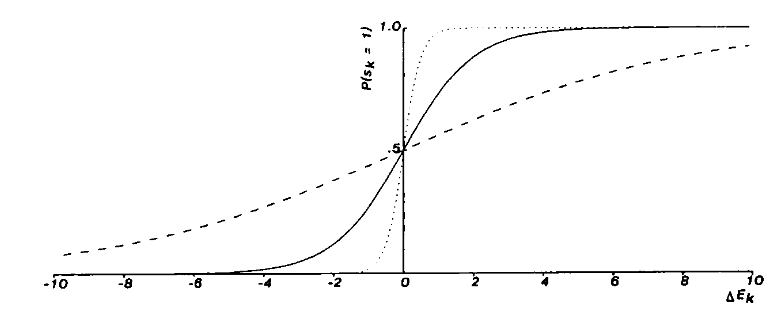
\includegraphics[width=0.6\textwidth]{images/temperature.png}
    \caption{The softmax function with different temperature values, T=1.0 (solid), T=4.0 (dashed), T=0.25 (dotted), Source: Ackey et al.\cite{ACKLEY.1985}}
    \label{fig:temperature}
\end{figure}

$$softmax: o(z)_i = \frac{e^{\beta z_i}}{\sum_{j=1}^K e^{\beta z_i}}$$

In figure \ref{fig:temperature} the softmax function is shown. A low temperature value leads to a peaky distribution, while a high temperature value leads to a more uniform distribution and therefore to more randomness.


% split paragraph in two parts
\paragraph{Top-K Sampling}
Top-K sampling \cite{Fan.13.05.2018} randomly selects from the top K tokens with the highest probability before applying the softmax function. Therefore the higher the K value, the more tokens are considered for sampling. Higher values increase output randomness. With Top-K equal to 1, the model behaves like greedy decoding.

\paragraph{Top-P Sampling}
The Top-P sampling \cite{Holtzman.22.04.2019} randomly selects from the smallest set of tokens whose cumulative probability exceeds the probability P. Therefore the higher the P value, the more tokens are considered for sampling. The outcomes gets more random. It is a generalization of Top-K sampling, where the number of tokens to sample from is not fixed.

\subsection{Prompting Techniques}
The Transformer architecture is not deterministic as shown in previous sections. Additionally LLMs have a high variance for its outputs too. The input prompt critically influences output quality. Therefore there are plenty of prompting techniques to stabilize desired outputs. Schulhoff created a taxonomy and recognized 58 LLM prompting techniques \cite{Schulhoff.06.06.2024}. We discuss four representative prompting techniques: Few-Shot, Zero-Shot, Chain-of-Thought (CoT), and Chain-of-Verification (CoVe). The list is not complete, but those are very commonly used and easy to implement.

\paragraph{Few-Shot vs. Zero-Shot}

\begin{figure}[h!]
    \centering
    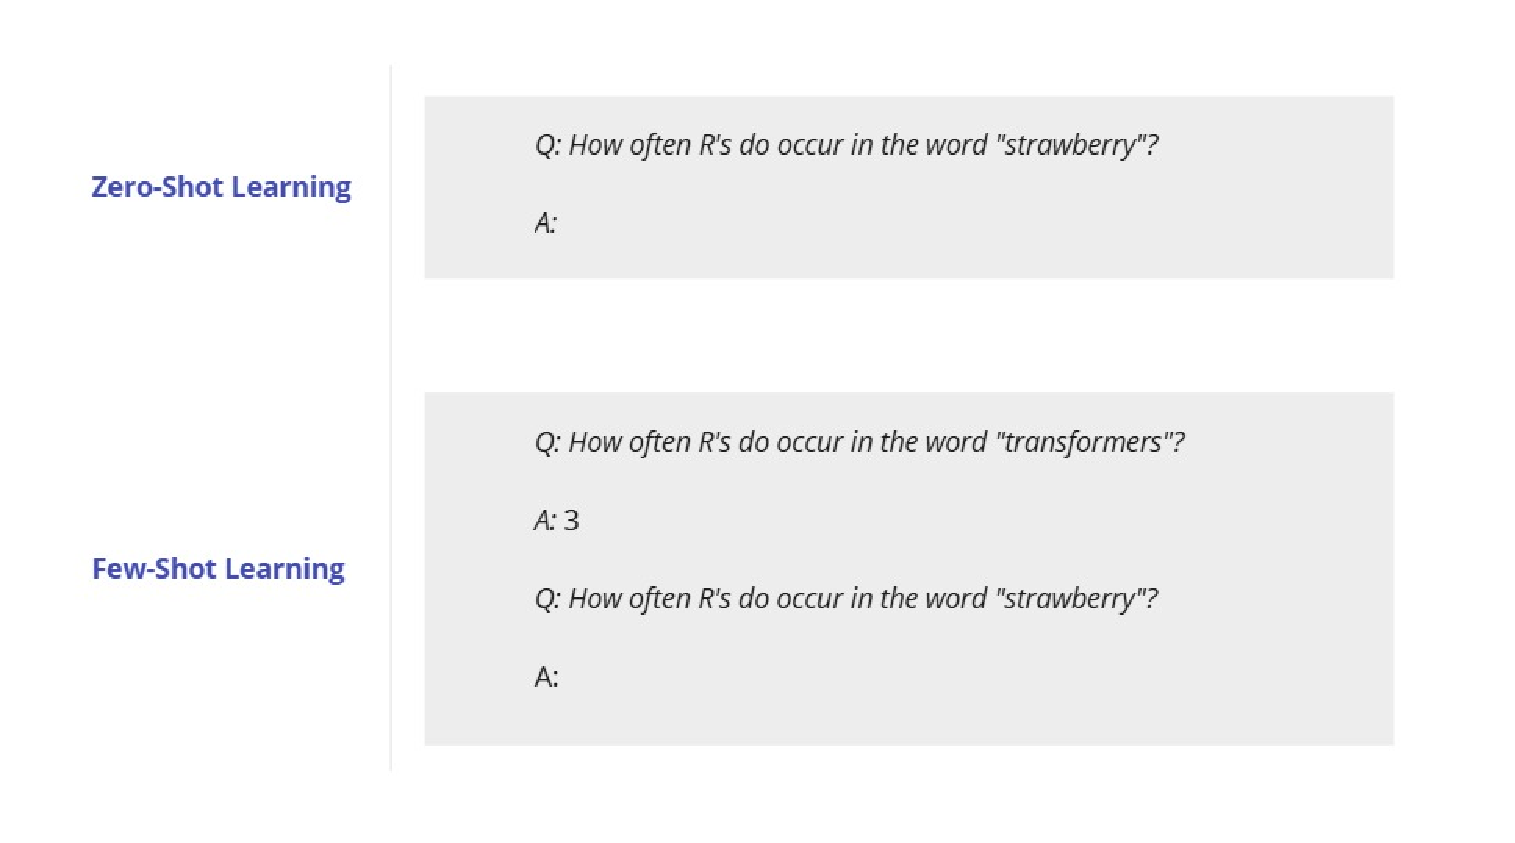
\includegraphics[width=\textwidth]{images/FewShot vs ZeroSHot.pdf}
    \caption{An example with a difficult query, that many LLM struggle, first without example (Zero-Shot) and below with one example (Few-Shot).}
    \label{fig:FewZeroShot}
\end{figure}


Few-Short prompting is a form of In-Context Learning (ICL), in which the prompt has examples of similar tasks to show the model how a task should be done. Brown showed that large models can leverage examples for various tasks \cite{Brown.28.05.2020}. Zero-Shot prompting refers then to prompting without showing examples before the task. Even though Few-Shot prompting might increase performance of LLMs, it comes with increased costs, as there are more tokens to process. An example of those prompting methods can be seen in figure \ref{fig:FewZeroShot}.

\paragraph{Chain-of-Thought}

\begin{figure}[h!]
    \centering
    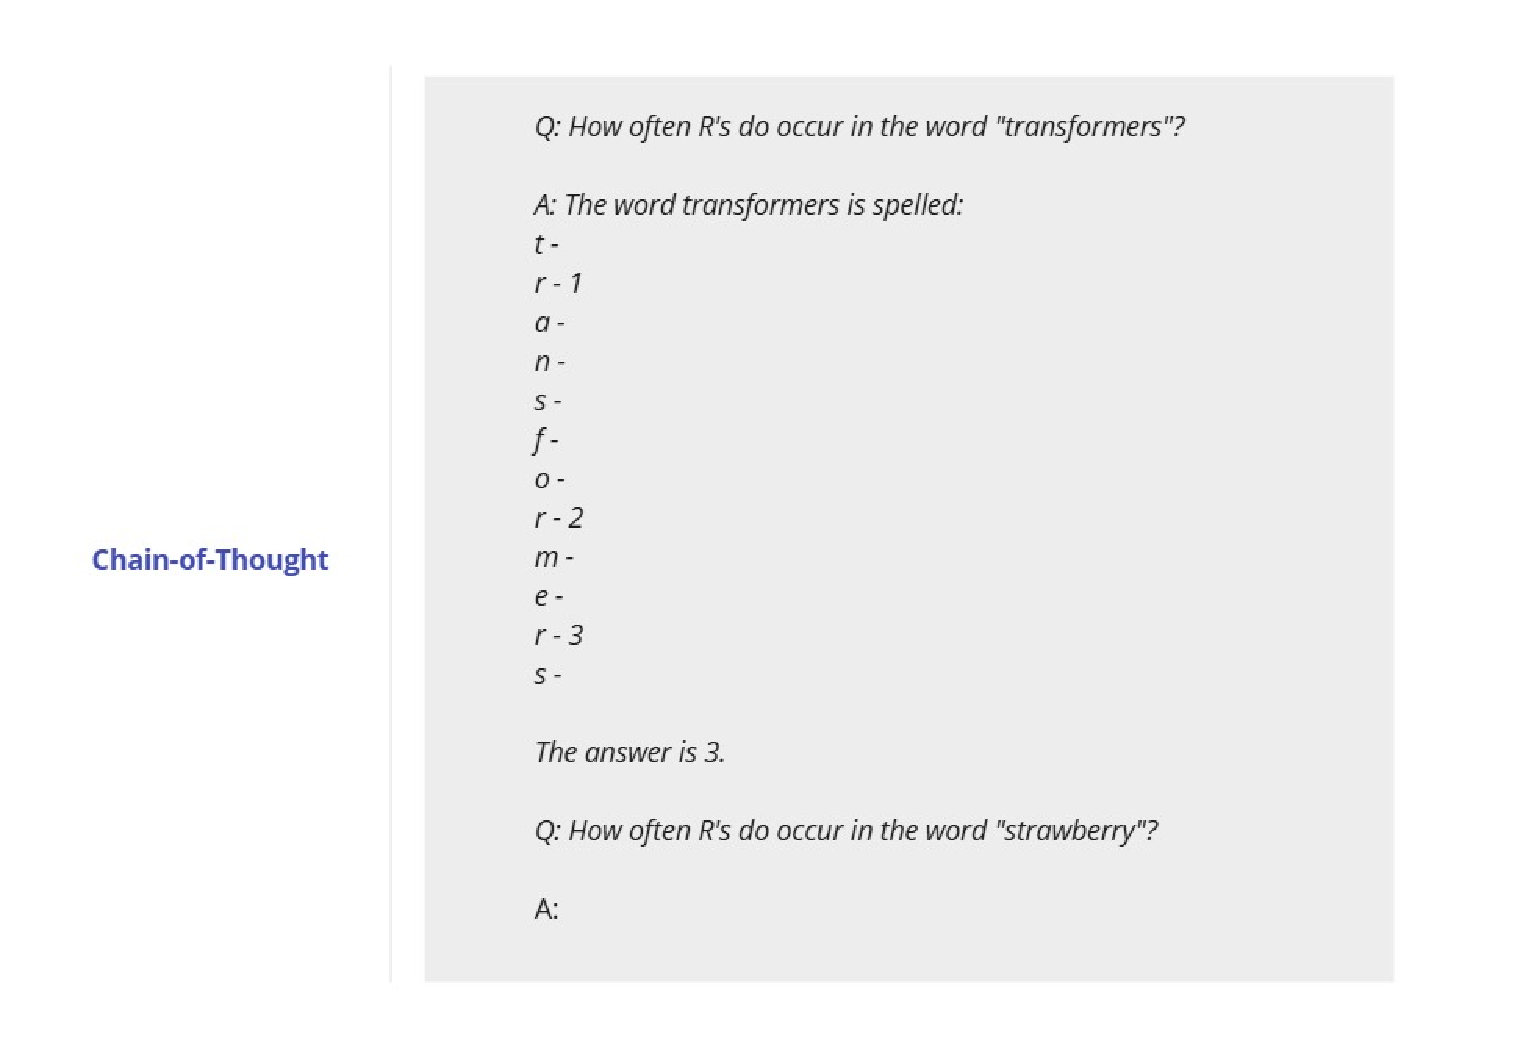
\includegraphics[width=\textwidth]{images/Chain-of-Thought.pdf}
    \caption{An Chain-of-Thought example with a difficult query, that many LLM struggle without prompting techniques}
    \label{fig:CoT}
\end{figure}


This method introduced by Wei leverages Few-Shot learning through simulating a written thought process in prior examples \cite{Wei.28.01.2022}. The LLM is therefore forced to take over this behaviour, which leads to more accurate outputs in reasoning and math problems. Schulhoff refers to it as the class of Thought Generation techniques \cite{Schulhoff.06.06.2024}. Figure \ref{fig:CoT} shows an example prompt.

\paragraph{Chain-of-Verification}


\section{Text Retrieval}\label{retrieval}
%!TEX encoding = UTF-8 Unicode

There are several types of text retrieval for RAG systems. \citet{Zhao.29.02.2024} classified four different types of retrieval techniques regarding how the retrieved information are passed to the generation. In this thesis I will only focus on query-based retrievals as they are the most common and widely used retrieval techniques. The other three types are latent-representative-based retrieval, logit-based and speculative retrieval.

Another categorization of text retrieval can be done by the type of retrieval. There are three main types of retrieval: sparse retrieval, dense retrieval and hybrid retrieval. Sparse retrieval is based on traditional information retrieval techniques like TF-IDF or BM25. Dense retrieval is based on transformers models and hybrid retrieval combines both sparse and dense retrieval techniques. Following I  will describe those techniques in more detail.
\subsection{Sparse Retrieval}
\label{sec:sparse_retrieval}

\paragraph{TF-IDF}
\label{sec:tfidf}

TF as shown in \citet{Manning.2009} refers to the term frequency of a term $t$ in a document $d$. The inverse document frequency (IDF) is calculated as the logarithm of the total number of documents $N$ divided by the number of documents containing the term $t$. Therefore the IDF factor is low for terms that occur in all documents and high for distinguishing terms that occur in frequently in a low number of documents. The position of the words is ignored.

$$\textit{TF-IDF}(t, d, D) = \textit{TF}(t, d) \cdot \textit{IDF}(t, D) = \textit{TF}(t, d) \cdot \log\left(\frac{N}{\textit{DF}(t, D)}\right)
$$

\paragraph{BM25}
\label{sec:bm25}

\citet{Manning.2009} showed several versions of it. One simpler one is defined as following.


$$BM25(t, d, D) = IDF(t, D) \cdot \frac{(k_1 + 1) \cdot TF_{t, d}}{k_1((1-b)+b \cdot \frac{L_d}{L_{ave}}) + TF_{t, d}}$$


The BM25 score is an advanced version of the TF-IDF score with two free parameters $k_1$ and $b$. The parameter $k_1$ is a scaling factor to determine how relevant term frequency is. The parameter $b$ is for document length scaling, reducing scores of long documents.

\subsection{Dense Retrieval}
\label{sec:dense_retrieval}

Dense Passage Retrieval as shown in \citet{karpukhin2020densepassageretrievalopendomain} utilizes Bidirectional Encoder Representation from Transformers (BERT, \citet{devlin2019bertpretrainingdeepbidirectional}). BERT can be seen as the encoders part of an sequence-to-sequence transformers architecture. Therefore it can be used to encode the text passages used as contexts at the classification token [CLS]. The text is thus mapped into an d-dimensional real-valued space with the assumption that semnatic similar passages are close to each other in this space. The query is also encoded into this space and the similarity between the mapped query vector and each passage vector is calculated. The similarity is calculated by the dot product or other similarity functions. The top-k similar passages are then selected and used for the generation.

Nowadays there are highly specialized embedding models, that are benchmarked and listed on the Huggingface MTEB as described in \citet{muennighoff2022mteb}. Even though the MTEB leaderboard suggests a best-of-all embedding model, there is no such thing. Embedding models are language- and domain-sensitive as \citet{Gao.18.12.2023} points out. 

\subsection{Hybrid Retrieval}
\label{sec:hybrid_retrieval}

Both sparse retrieval techniques TF-IDF and BM25 are good for keyword specific searches, but perform poorly on a semantic comparison of documents and query. Encoders like BERT were trained for understanding languages and are thus good for a semantic understanding. Often it is not trivial to dertermine if a text retrieval needs a keyword-relevant sparse retrieval or dense retrieval considering semantics. 

Hybrid models calculate both dense retrieval and sparse retrieval scores and multiply it then with factor $\alpha$ and $1-\alpha$ respectively. An factor $\alpha=1$ results in using only dense retrieval. There is no universal performant value for $\alpha$. Therefore this is a hyperparamter tuning parameter that needs to get optimizied.



\section{Retrieval-Augmented Generation Systems}\label{rag}
Large language models suffer from several fundamental issues, which are not entirely solvable through training or prompt engineering. 
\citet{Gao.18.12.2023} stated that LLMs have significant limitations in knowledge-intesive or domain-specific tasks. Missing or unsufficient amount of information on a specific subject while training lead to wrong answers. For large language models this is called \textit{hallucinations} as defined in \citet{Huang.2023}. For retrieval-augmented generation systems (RAGs) the term hallucinations is defined for stating information without context. \citet{Rashkin.} defined hallucinations as any information that is neither inferable from nor stated by an external document. In this thesis I will use the definition for RAG systems. 

Factual wrong output from an LLM can have several reasons. The required information to answer this question can be private, stored on a database that is not accessible during training. Another reason might be that training or fine-tuning the model is expensive and thus done less frequent. Therefore the required information can be published more recently then the last training run. All those problems can be solved if the LLM is not used for the answer itself, but rather used for building a coherent text passage given a question and its answer. Then a database would store all relevant information and would be updated as frequent as required. At inference time the prompt is used to determine relevant chunks of documents within the database, which are then used for the generation of the answer.

This concept is very successful as \citet{Shuster.} showed. Factual wrong outputs are reduced and open-domain conversational capabilities are increased. \citet{Yu.2024} concluded that this improves the reliability and richnes of the produced content. \citet{Chen.2024} stated that external knowledge would be the key for resolving the above stated problems of LLMs, which make them more accurate and reliable.

There is a high variety in architectures and approaches for retrieval-augmented generation models. In this section, I will give an overview of the most common approaches and architectures and start with the most basic ones. The section will follow the definition of RAGs in \citet{Gao.18.12.2023} with naive RAGs, advanced RAGs, a modular architecture, and special cases. 

\subsection{Naive RAGs}
\label{sec:naive_rags}
Naive RAGs can be seen as the most basic form of a retrieval-augmented generation system. The core idea behind this concept is to give all relevant context for answering a question or solving a task into the prompt for the large language model. Then the LLM is only used for generating a coherent answer. Therefore it is required to ingest relevant data for the given use case beforehand. The system then retrieves relevant chunks or documents of this data at inference time. 


\begin{figure}[h!]
    \centering
    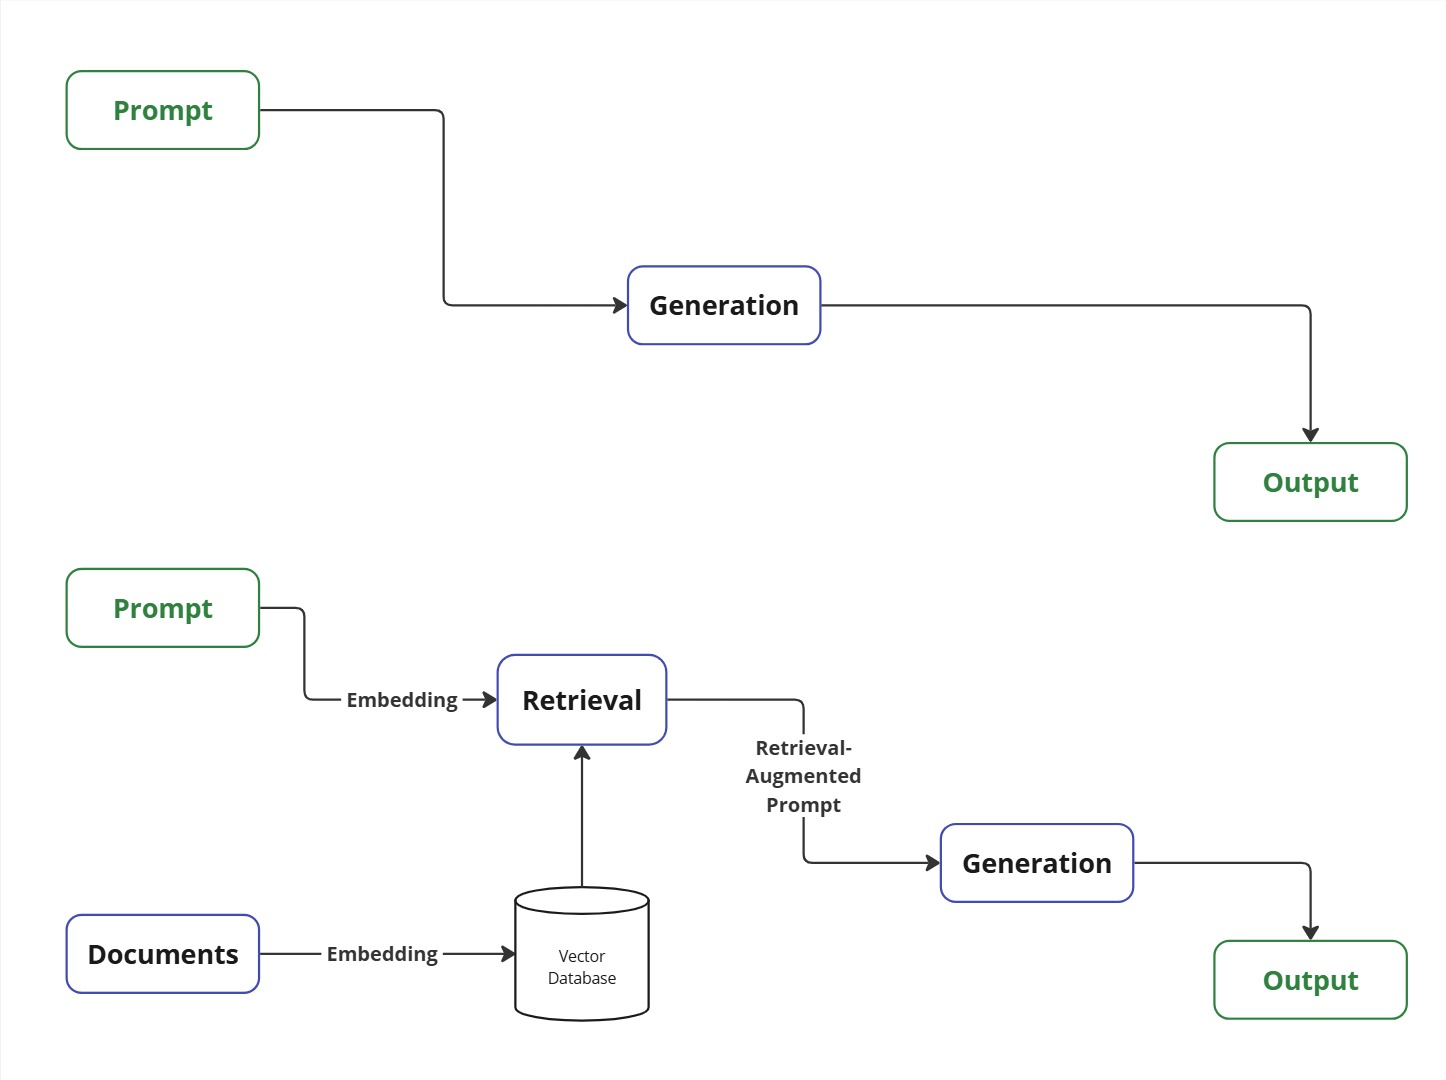
\includegraphics[width=\textwidth]{images/LLM-vs-RAG.jpg}
    \caption{Comparison of the process to the prompt, above a standalone LLM that has a prompt and generate a response, below a RAG system that performs on a given set of documents an embedding or indexing and searchs for the most similar documents for a given prompt at inference time. Both prompt and documents are used for the generation process.}
    \label{fig:naive_rag}
\end{figure}

This procedure can be seen in figure \ref{fig:naive_rag}. In the literature the generation process is often refered as \textit{read}, because it reads the prompt and the provided context. In \citet{Gao.18.12.2023} they define the naive RAG system as \textit{Retrieve-Read}. The retrieval can be done with sparse retrieval (TF-IDF, BM25), dense retrieval (DPR) or a hybrid version as showed in section \ref{retrieval}. 

\begin{figure}[h!]
    \centering
    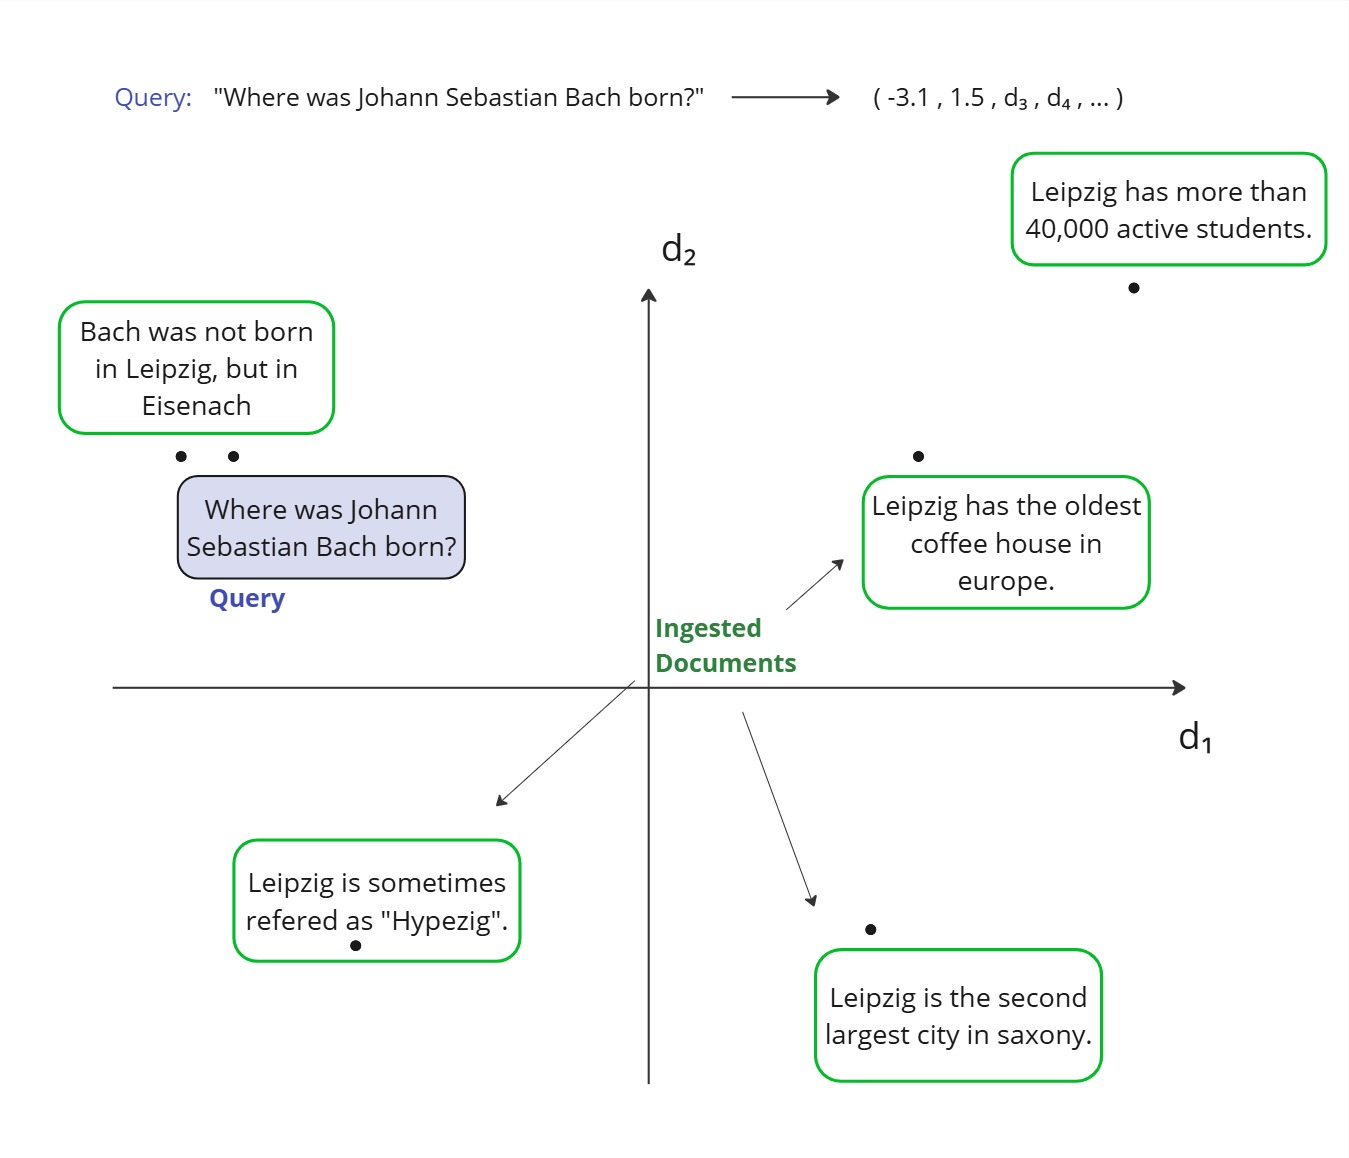
\includegraphics[width=\textwidth]{images/VectorDB.jpg}
    \caption{A vector space including mapped facts (documents) and a user query. The query and its correct answer have similar vectors}
    \label{fig:vectorDB}
\end{figure}


Before the system can be used, it is necessary to ingest data. The ingestion process includes preprocessing and selection of data, that users are likely to need for their questions or use-cases. Therefore it is relevant to know the user base. It is not feasible nor efficient to ingest all availlable data. The data is transformed into documents or chunks of documents. There are multiple ways to do this, which are described in advanced techniques. As described in \ref{sec:dense_retrieval}, the chunks are then encoded and mapped into a d-dimensional real-valued vector space. There is a simplistic minimal example of a vector space in figure \ref{fig:vectorDB}. The documents gets mapped in different loactions within the space. The assumption is, that the embedding model will map correct answers to the corresponding queries. In reality there will be more documents close to each other, documents and queries are longer or more complex and each query will return the "Top-K" chunks or documents, which are not always as relevant as in this example. Top-K can be seen as hyperparamter for the system. 

The vectors are then stored in so called vector databases. Such databases are specialized and include functionalities like inverted indices, clustering of precomputed vector similarities, approximate nearest neighbor algorithm, hierarchical navigable small world and quantizations, which will not be covered in this master thesis.  


\citet{Gao.18.12.2023} listed several drawbacks for naive RAGs. The basic retrieval suffers from unsufficient recall and precision scores leading in irrelevant documents, missing context and bias. The integration of the provided context is a challenging process. The generator often overrelies on the augmented information, by just repeating the retrieved content and missing insightful conclusions. Therefore this simplistic form of RAG needs advanced techniques to overcome those issues. 

\subsection{Advanced RAGs}
\label{sec:advanced_rags}

There is no strict definition of advanced versions of retrieval-augmented generation systems. The term describes a loose bundle of techniques to improve the quality of such systems. Following is a list, which items I will explain in greater details afterwards.

\paragraph{Chunking}
\label{sec:chunk}
% graphic for techniques, such as overlap, fixed sized (sliding window approach), semantic chunks, ...
For understanding the necessarity of chunking it is helpful to illustrate it with a following example. Let us use a sentence from \citeauthor{LeipzigWikipedia.2025} for Leipzig from \citeyear{LeipzigWikipedia.2025}. In the section "Music" there is the following sentence. 

\begin{quote}
    "Johann Sebastian Bach spent the longest phase of his career in Leipzig, from 1723 until his death in 1750, conducting the Thomanerchor (St. Thomas Church Choir), at the St. Thomas Church, the St. Nicholas Church and the Paulinerkirche, the university church of Leipzig (destroyed in 1968)."
\end{quote}

If there are thousands of wikipedia pages or websites to process, then this can not be splitted manually. What is the document or a good chunk in this context. If the query asks if Johann Sebastian Bach lived in Leipzig, then embedding the whole sentence would not guarantee a high similarity vector score in the retrieval process. This differs from domain to domain. While chunking facts from sentences might be a valid strategy for wikipedia, processing internal contracts in a large company would need less granular chunking. 

Therefore there are several chunking techniques to consider for tuning the RAG-system. Fixed-Size chunking splits a document after a fixed size of characters, e. g. every 400 characters a chunk ends and a new one starts. The sliding window approach adds a overlap of few characters. Semantic Chunking splits with prior defined characters such as "\textit{$\backslash n$, $\backslash\backslash n$ or <br>}". There are also special use-case techniques such as Markdown, JSON, HTML and programming code chunkers. Almost all presented chunking techniques are offered in typical libraries e. g. Llama-Index (\citet{Liu_LlamaIndex_2022}) or Langchain (\citeauthor{Chase_LangChain_2022}).

Additional to advanced chunking, it is recommended to enrich the resulting documents with metadata, which can be used at inference time for filtering. 

% ToDo: 
% - Just Write them Down!
% - Drawbacks
% - Point of Failures in RAGs
% - Überleitung zu Evaluation

\paragraph{Rewrite}
\label{sec:rewrite}
% Query Rewriting, Query Transformation, Query Expansion (see. papers)

\paragraph{Rerank}
\label{sec:rerank}
% Reranking Techniques, Lost-in-The-Middle?, Diversity Ranking, ... 

\paragraph{Iterative RAGs}
\label{sec:iterative}
% Short description with graphic

\paragraph{Recursive RAGs}
\label{sec:recursive}
% Short description with graphic

\paragraph{Adaptive RAGs}
\label{sec:adaptive}
% Short description with graphic

\subsection{General Modular RAG}
\label{sec:modular_rag}
% The core idea behind it, to be as flexible as possible and bridge to special cases

\subsection{Special Cases}
\label{sec:special_cases}
% short list of special cases

\subsection{Drawbacks of RAGs}
\label{sec:drawbacks}


% Appendix
%\appendix
%\chapter{Experiment Results}

% Bibliography
\bibliographystyle{plainnat} % requires package natbib. An alternative is apalike
\bibliography{literature.bib}    % load file literature.bib

\end{document}
